\chapter{Kapitel}
\label{chap:kap}

\section{Abschnitt}
\label{sec:ab}
Text
\begin{itemize}
\item Liste
\end{itemize}
\begin{figure}[!htb]
\centering
\begin{subfigure}[t]{0.8\linewidth}
\includegraphics[width=\textwidth]{}
\caption{Unterschrift}
\label{abb:u}
\end{subfigure}
\begin{subfigure}[t]{0.8\linewidth}
\includegraphics[width=\textwidth]{}
\caption{Unterschrift}
\label{abb:tes2}
\end{subfigure}
\begin{subfigure}[t]{0.8\linewidth}
\includegraphics[width=\textwidth]{}
\caption{Unterschrift}
\label{abb:tes3}
\end{subfigure}
\caption{Unterschrift}
\label{abb:test}
\end{figure}


\begin{figure}[!ht]
\centering
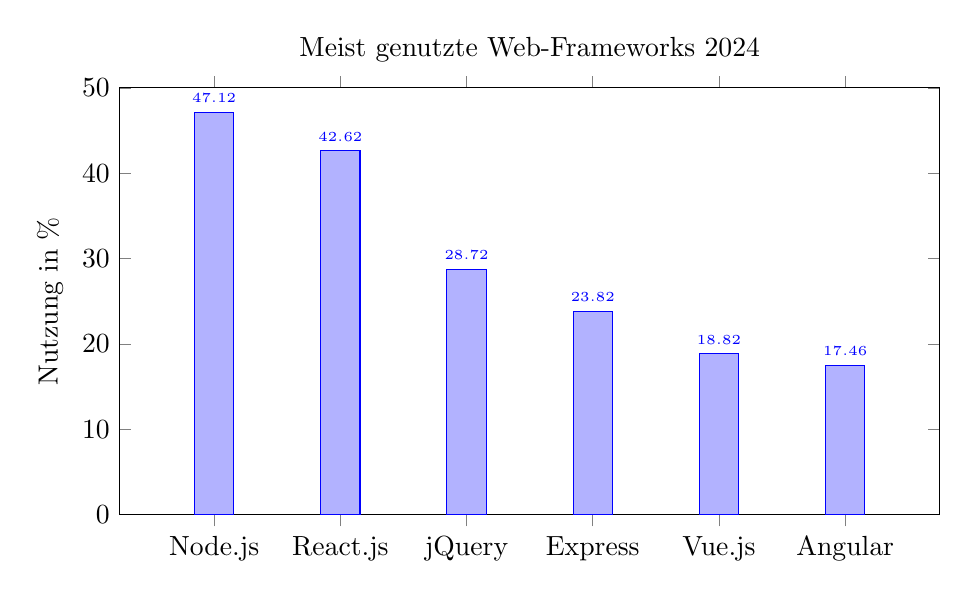
\begin{tikzpicture}
\begin{axis}[
    ybar,
    bar width=0.5cm,
    width=12cm,
    height=7cm,
    ymin=0,
    ymax=50,
    ylabel={Nutzung in \%},
    symbolic x coords={Node.js, React.js, jQuery, Express, Vue.js, Angular},
    xtick=data,
    nodes near coords,
    nodes near coords align={vertical},
    every node near coord/.append style={font=\tiny},
    enlarge x limits=0.15,
    title={Meist genutzte Web-Frameworks 2024}
]
\addplot coordinates {
    (Node.js, 47.12)
    (React.js, 42.62)
    (jQuery, 28.72)
    (Express, 23.82)
    (Vue.js, 18.82)
    (Angular, 17.46)
};
\end{axis}
\end{tikzpicture}
\caption{Säulendiagramm: Meist genutzte Web-Frameworks laut weltweiten Entwicklern, Onlineumfrage Stack Overflow, Juli 2024 }
\end{figure}


\begin{longtblr}[
    caption={Tabelle mit der Übersicht von Testverfahren},
    label={tab:verf},
    headsep=\abovecaptionskip
    ]
    {
    width=0.9\textwidth,
    colspec={X[1,l]Q[3,c]rl}}
    
    \toprule	
    Testverfahren   & Beschreibung   \\
    \midrule
    A  & Beschreibung\\
     \midrule     
    \bottomrule
\end{longtblr}
\cite{paper3:2024}
\(
% \begin{lstlisting}[DEF]
% Def
% \end{lstlisting}
% \begin{lstlisting}
% \end{lstlisting}

\begin{enumerate}
\item ein Punkt
\end{enumerate}

\texttt{<table>}
\enquote{Utility}-Klassen
\textit{test}
\gls{Abkürzung}
\url{https://bpb.de/}
\begin{figure}[!ht]
\centering
%\includegraphics[width=1.0\textwidth]{}
\caption{Unterschrift}
\label{abb:tailw}
\end{figure}

\section{Endergebnis}
\label{sec:end}

\subsection{Codegen}
\label{sub:cod}

\begin{itemize}
\item einPunkt
\end{itemize}


\begin{figure}[!ht]
\centering
\includegraphics[width=1.0\textwidth]{Bilder/App2.png}
\caption{Screenshot der Kalenderapp: Formular}
\end{figure}
\begin{figure}[!ht]
\centering
\includegraphics[width=1.0\textwidth]{Bilder/App3.png}
\caption{Screenshot der Kalenderapp: Termin}
\end{figure}
\ac{Abkürzung}
\begin{figure}[tbp]
\centering
%\includegraphics[width=1.0\textwidth]{}
\caption{Unterschrift}
\label{}
\end{figure}










